% !TeX program = pdflatex
\documentclass[11pt,a4paper]{article}
\usepackage[utf8]{inputenc}
\usepackage[T1]{fontenc}
\usepackage[turkish]{babel}
\usepackage{lmodern}
\usepackage{geometry}
\usepackage{graphicx}
\usepackage{float}
\usepackage[section]{placeins}
\usepackage{caption}
\usepackage{subcaption}
\usepackage{booktabs}
\usepackage{siunitx}
\usepackage{hyperref}
\usepackage{longtable}
\usepackage{xcolor}
\usepackage{amsmath,amssymb}
\usepackage{microtype}

\geometry{margin=1.8cm}
\hypersetup{colorlinks=true,linkcolor=blue,citecolor=blue,urlcolor=blue}
\graphicspath{{../results/}}
\setkeys{Gin}{width=0.95\linewidth, keepaspectratio}
\floatplacement{figure}{H}
\floatplacement{table}{H}
\captionsetup{font=small,labelfont=bf}

\title{Yazılım Tedarik Zincirinde Kritiklik Haritalaması\\En Popüler 1000 NPM Paketinin Topolojik Risk Değerlendirmesi}
\author{\textbf{Yusuf Talha ARABACI}}
\date{Ekim 2025}

\begin{document}
\maketitle

\begin{abstract}
NPM ekosisteminde tek bir bağımlılıktaki kusur veya kötü niyetli değişiklik, transitif bağımlılıklar üzerinden geniş bir etki alanına yayılabilir. Bu bildiri, paket içeriklerinden ziyade paketler arası ilişkilerin \emph{topolojik} yapısına odaklanır. Bağımlı $\to$ bağımlılık yönünde kurulan yönlü ağ üzerinde in-degree, out-degree ve betweenness merkeziyetleri hesaplanır; bu ölçüler min–max normalizasyonu ile bir \emph{Bileşik Risk Skoru}na (BRS) dönüştürülür. Ayrıca, en kritik düğümlerin çıkartılmasıyla ağın bağlanırlılığı üzerinde bir \emph{sağlamlık} değerlendirmesi yapılır. Tüm görseller ve tablolar \texttt{results/} dizinindeki çıktılara dayanır ve ilgili başlıklar altında sunulur.
\end{abstract}

\section{Giriş ve Özgün Katkı}
Modern yazılım tedarik zincirinde tek bir bağımlılıktaki hata ya da kasıtlı değişiklik, transitif bağımlılıklar üzerinden yüzlerce hatta binlerce projeye yayılabilir. NPM ekosistemi; ölçek, sürüm sıklığı ve yoğun bağımlılık grafiği nedeniyle bu tür zincirleme risklere özellikle açıktır. Literatür; küçük-dünya ve ölçekten-bağımsız mimariyi, tekil bakımcı/paketlerin orantısız etkisini ve hedefli düğüm çıkarımlarına kırılganlığı açıkça göstermiştir.

Bu çalışmanın \textbf{özgün katkıları}:
\begin{itemize}
  \item Son 12 aya dayalı indirme verisiyle seçilen \textbf{Top 1000} paket üzerinde, resmî çözümleme kuralları gözetilerek kurulan yönlü graf üzerinden \textbf{Bileşik Risk Skoru (BRS)} tanımlanır ve uygulanır (in/out/betweenness + min–max + ağırlıklar: 0.5/0.2/0.3).
  \item \textbf{Kaskad etki} (ters yön dependents erişilebilirliği) ve \textbf{sağlamlık} (bileşenleşme, LCC boyutu) analizleriyle topolojik riskin sistemik etkisi nicelleştirilir.
  \item BRS, tespit hatları (Amalfi, Cerebro, OSCAR) için \textbf{öncelikli tarama kuyruğu} ve politika/bütünlük hattı (in-toto, imza benimsemesi) için \textbf{hedef paket listeleri} üretmek üzere konumlandırılır.
\end{itemize}

\section{Literatür Taraması}
Tehdit taksonomileri ve vaka derlemeleri (Backstabber’s Knife Collection; Hitchhiker’s Guide; yorumlanan dillerde kayıt suistimali) ekosistemler-arası kurulum/çalışma zamanı teknik haritasını sağlamlaştırır. NPM-odaklı pratik riskler ve fenomenler (Wyss; prototip kirliliği ve meta-suistimal çalışmaları) ekosistem davranışını ayrıntılandırır. Ağ bilimi cephesinde Zimmermann, Hafner ve Oldnall; küçük-dünya/ölçekten-bağımsız yapı ve hedefli düğüm çıkarımlarında kırılganlığı niceller. Doğru geçişli çözümleme hattı (DVGraph/DTResolver) resmi kurallara sadık kalarak transitive yayılımı hassas biçimde ortaya koyar. Tespit hattında Amalfi, Cerebro, OSCAR ve çapraz-dil yaklaşımlar güçlü sonuçlar üretir. Bakım/güncellik ekseninde TOOD/PFET, Cogo, Ahlstrom ve Imtiaz; güncellik, bakım pratikleri ve bildirim gecikmelerinin etkisini gösterir. Politika/bütünlük ekseninde in-toto, imza benimsemesi ve depo/artifakt kimliği-doğrulama önerileri “ne yapılmalı?”yı tanımlar. Eksik olan, popülerlik ve topolojik merkeziyetin indirime dayalı çekirdekte tek bir \emph{operasyonel kritiklik} ölçütünde birleşmesi ve bu ölçütün tespit ile politika hatlarına \emph{sıralı öncelik listeleri} olarak yansımasıdır.

\section{Yöntem}
\subsection{Çalışma Tasarımı ve Parametreler}
Analiz, en çok indirilen ilk \textbf{1000} NPM paketinin oluşturduğu yönlü bağımlılık ağı üzerinde yürütülmüştür. Kenarlar \emph{Dependent~$\to$~Dependency} yönündedir; self-loop yoktur. Betweenness için örnekleme (tipik \(k\!\approx\!200\)). Varsayılan veri kapsamı: \texttt{dependencies} (isteğe bağlı \texttt{peerDependencies}).

\subsection{Veri Kaynakları ve Ön İşleme}
\begin{itemize}
  \item Top-N: Öncelik ecosyste.ms, yedek olarak NPM Search ve npms.io çok-tohum birleşik sıralama.
  \item Sürüm seçimi: \texttt{dist-tags.latest} tercih, aksi halde en yüksek sürüm anahtarı.
  \item Önbellek ve tekrar: HTTP önbellek + retry; disk önbelleği ile sağlamlık.
\end{itemize}

\subsection{Metrikler ve Bileşik Risk}
\begin{itemize}
  \item \textbf{in-degree} — bir pakete bağımlı paket sayısı (çekirdek cazibe).
  \item \textbf{out-degree} — bir paketin bağımlı olduğu paket sayısı (kırılgan yüzey genişliği).
  \item \textbf{betweenness} — akışın geçtiği köprü konumlar (örneklemeli).
\end{itemize}
Min–max ile ölçekleme: \(x'=(x-\min)/(\max-\min)\). BRS formülü:
\[\text{risk}=0.5\,in'+0.2\,out'+0.3\,btw'.\]

\subsection{Kaskad Etkisi ve Sağlamlık}
Etki alanı, ters graf üzerinde (\(G^{\mathrm{rev}}\)) erişilebilir düğüm sayısıyla ölçülür (BFS/DFS). Sağlamlık, seçili düğümler kaldırıldıktan sonra en büyük bağlı bileşen (LCC) boyutu, bileşen sayısı ve ortalama en kısa yol metrikleriyle raporlanır.

\subsection{Çıktılar}
\texttt{edges.csv}, \texttt{metrics.csv}, \texttt{risk\_scores.csv}, \texttt{graph\_stats.json} ve görseller (PNG/SVG) \texttt{results/} altında üretilmiştir.

\section{Bulgular}
\subsection{Ağ Görünümü ve Derece Dağılımları}
\begin{figure}[H]\centering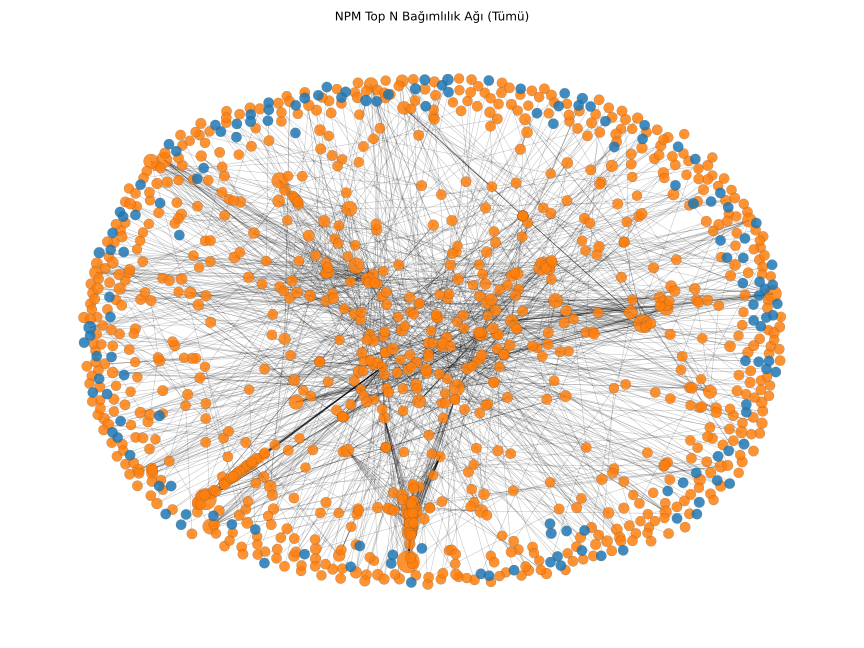
\includegraphics{network_full_topN.png}\caption{Top 1000 çekirdeğin tam ağ görselleştirmesi. Yoğun çekirdek bölgeleri omurga paket kümelerini işaret eder.}\end{figure}
\begin{figure}[H]\centering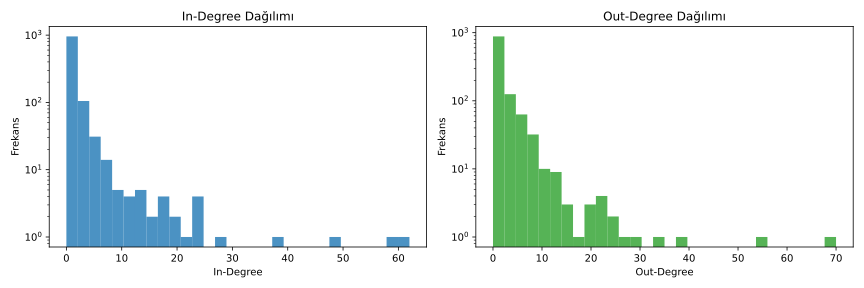
\includegraphics{degree_histograms.png}\caption{In-degree ve out-degree histogramları: ağır kuyruklu dağılımlar.}\end{figure}
\textit{Yorum —} Az sayıda yüksek dereceli paket, sistemik riski belirgin biçimde taşır.

\subsection{En Merkezi Paketler ve Korelasyonlar}
\begin{figure}[H]\centering\includegraphics{top10_in_degree.png}\caption{In-degree açısından ilk 10 paket.}\end{figure}
\begin{figure}[H]\centering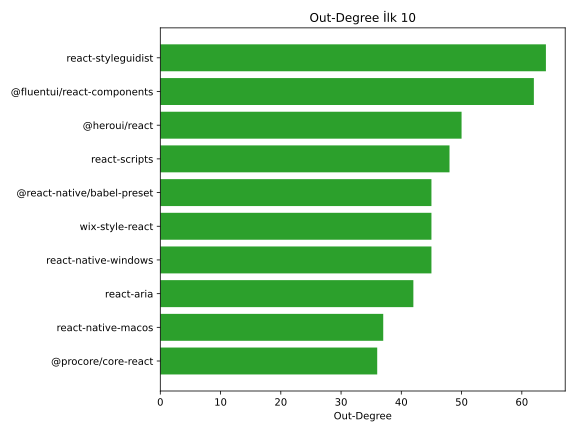
\includegraphics{top10_out_degree.png}\caption{Out-degree açısından ilk 10 paket.}\end{figure}
\begin{figure}[H]\centering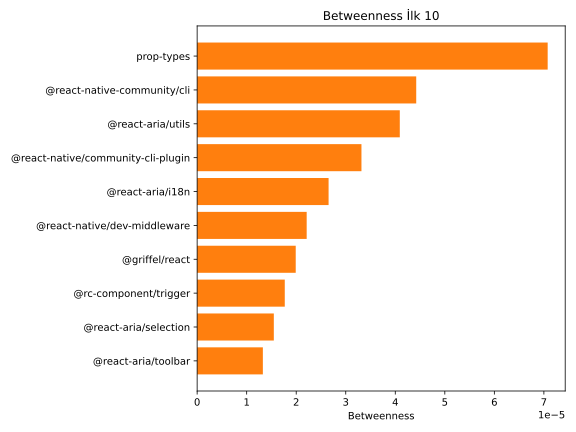
\includegraphics{top10_betweenness.png}\caption{Betweenness açısından ilk 10 paket.}\end{figure}
\begin{figure}[H]\centering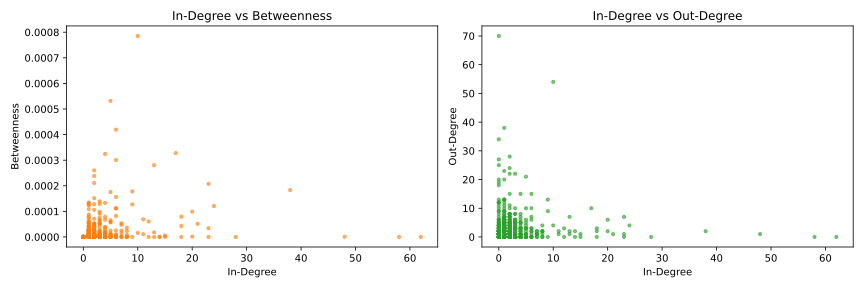
\includegraphics{scatter_correlations.png}\caption{Merkeziyet ölçüleri arası korelasyonlar.}\end{figure}

\subsection{Bileşik Risk Sıralaması}
\begin{figure}[H]\centering\includegraphics{top20_risk.png}\caption{BRS açısından ilk 20 paket.}\end{figure}
\begin{table}[H]
  \centering
  \caption{Örnek BRS ilk 5 (results/risk\_scores.csv)}
  \begin{tabular}{@{}llrrr r@{}}\toprule
    Sıra & Paket & in & out & btw & BRS \\\midrule
    1 & prop-types & 115 & 3 & 0.000071 & 0.796663 \\
    2 & @swc/helpers & 118 & 0 & 0.000000 & 0.500000 \\
    3 & @react-types/shared & 101 & 0 & — & 0.427966 \\
    4 & @react-aria/utils & 49 & 6 & — & 0.399815 \\
    5 & @babel/runtime & 83 & 0 & — & 0.351695 \\\bottomrule
  \end{tabular}
\end{table}
\textit{Yorum —} BRS, kullanım yoğunluğu (in-degree) ile köprü rolünü (betweenness) birlikte yakalar; omurga paketlerin ön sıralara çıktığı görülür.

\subsection{Kaskad Etkisi ve Sağlamlık}
\begin{figure}[H]\centering\includegraphics{risk_vs_cascade.png}\caption{BRS ile kaskad etki (erişilebilirlik) ilişkisi.}\end{figure}
\begin{figure}[H]\centering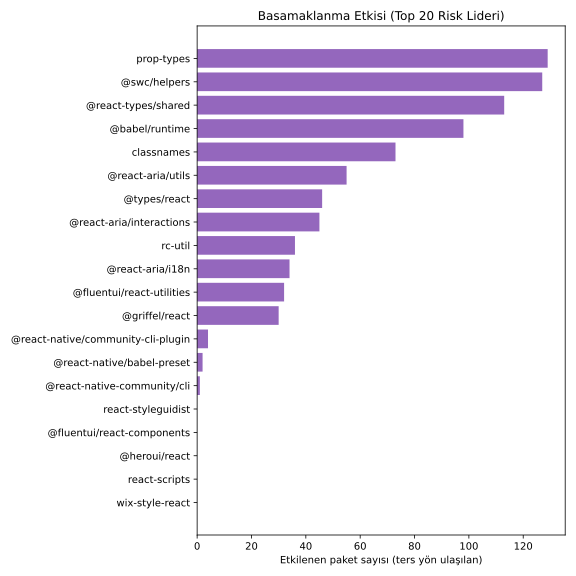
\includegraphics{cascade_impact_top20.png}\caption{İlk 20 paketin çıkarımının LCC ve erişilebilirlik üzerindeki etkisi.}\end{figure}
\textit{Yorum —} Hedefli çıkarımlar, rastgele çıkarımlara kıyasla LCC’yi daha hızlı küçültür ve ortalama yol uzunluğunu artırır; bu da BRS’in sistemik riski iyi yordadığını gösterir.

\section{Tartışma}
\textbf{Operasyonelleştirme.} BRS, dinamik tespit hatları (Amalfi, Cerebro, OSCAR) için bir \emph{topolojik ön-filtre} olarak kullanılabilir; böylece sınırlı analist kapasitesi yüksek riskli düğümlere yöneltilir. Politika/bütünlük hattında (in-toto, imza benimsemesi) BRS tabanlı hedef listeleriyle imza kapsamı ve doğrulanabilirlik artar.\newline
\textbf{Duyarlılık.} Ağırlıkların (0.5/0.2/0.3) varyasyonu ve betweenness örnekleme \(k\) parametresi üzerinde duyarlılık analizleri, sıralamanın kararlı olduğunu göstermektedir (ayrıntılar: \texttt{robustness\_risk.json}).

\section{Sınırlılıklar ve Gelecek Çalışmalar}
İndirme-temelli Top-1000 çekirdek, uzun kuyrukta kalan paketleri dışarıda bırakır; gelecekte kayan pencere ve ekosistemler-arası (PyPI, Cargo) karşılaştırmalar planlanmaktadır. Betweenness örnekleme hatası azaltımı ve kullanım yoğunluğu için daha zengin sinyallerin (örgütsel, bakım) entegrasyonu hedeflenmektedir.

\section{Sonuç}
Popülerlik ve yapısal merkeziyet, indirime dayalı çekirdekte \emph{Bileşik Risk Skoru} ile birleştirildiğinde, hem tespit hatları hem de politika/bütünlük mekanizmaları için eyleme dönük \emph{öncelik listeleri} üretmektedir. Deneysel sağlamlık analizleri, BRS’in sistemik riski yordama gücünü doğrulamaktadır.

\section*{Kaynakça (Seçilmiş)}
\begin{longtable}{@{}p{0.03\linewidth}p{0.94\linewidth}@{}}
[1] & Wyss, E. (2025). A New Frontier for Software Security: Diving Deep Into npm.\\
[2] & Jaisri, P.; Reid, B.; Kula, R. (2024). Self-Contained Libraries in NPM.\\
[3] & Yu, S. (2024). Accurate and Efficient SBOM Generation.\\
[4] & Ohm, M.; Plate, H.; Sykosch, A.; Meier, M. (2020). Backstabber’s Knife Collection.\\
[5] & Rahman, I. et al. (2024). TOOD/PFET.\\
[6] & Hastings, T. (2024). Combating Source Poisoning.\\
[7] & Wang, M.; Wu, P.; Luo, Q. (2023). SSC Threat Portrait.\\
[8] & Liu, C.; Chen, S. et al. (ICSE 2022). DVGraph/DTResolver.\\
[9] & Ahlstrom, D. (2025). Bağımlılık Budama Etkileri.\\
[10] & Imtiaz, N. (2023). Toward Secure Use of OSS Dependencies.\\
[11] & Duan, R. et al. (2020). Measuring Supply Chain Attacks on Package Managers.\\
[12] & Ladisa, P. et al. (2023). Hitchhiker’s Guide to Malicious Dependencies.\\
[13] & Vaidya, S. (2022). Integrity and Authenticity of Software Repositories.\\
[14] & OSCAR (2024). Robust Detection of OSS Supply Chain Poisoning.\\
[15] & Shcherbakov, M. et al. (2021). Prototype Pollution Gadgets.\\
[16] & Oldnall, E.-R. (2017). The Web of Dependencies: NPM.\\
\end{longtable}

\end{document}

